% This file was created with tikzplotlib v0.10.1.
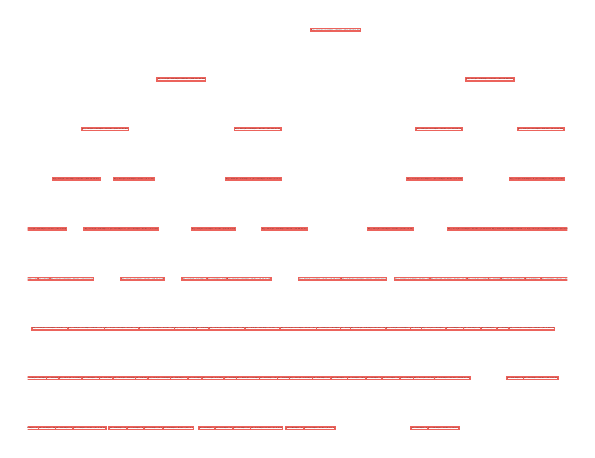
\begin{tikzpicture}

\definecolor{darkgray176}{RGB}{176,176,176}
\definecolor{tomato2369992}{RGB}{236,99,92}

\begin{axis}[
hide x axis,
hide y axis,
tick align=outside,
tick pos=left,
x grid style={darkgray176},
xmin=0, xmax=1,
xtick style={color=black},
y grid style={darkgray176},
ymin=0, ymax=1,
ytick style={color=black}
]
\draw (axis cs:0.0163934426229508,0.0555555555555556) node[
  scale=0.05,
  fill=white,
  draw=tomato2369992,
  line width=0.6pt,
  inner sep=3.6pt,
  text=black,
  rotate=0.0,
  align=center
]{gini = 0.341
samples = 699
value = [548, 3, 0, 148]};
\draw (axis cs:0.0491803278688525,0.0555555555555556) node[
  scale=0.05,
  fill=white,
  draw=tomato2369992,
  line width=0.6pt,
  inner sep=3.6pt,
  text=black,
  rotate=0.0,
  align=center
]{gini = 0.46
samples = 704
value = [455, 1, 2, 246]};
\draw (axis cs:0.0819672131147541,0.0555555555555556) node[
  scale=0.05,
  fill=white,
  draw=tomato2369992,
  line width=0.6pt,
  inner sep=3.6pt,
  text=black,
  rotate=0.0,
  align=center
]{gini = 0.493
samples = 281
value = [189, 19, 11, 62]};
\draw (axis cs:0.114754098360656,0.0555555555555556) node[
  scale=0.05,
  fill=white,
  draw=tomato2369992,
  line width=0.6pt,
  inner sep=3.6pt,
  text=black,
  rotate=0.0,
  align=center
]{gini = 0.7
samples = 528
value = [175, 31, 154, 168]};
\draw (axis cs:0.180327868852459,0.0555555555555556) node[
  scale=0.05,
  fill=white,
  draw=tomato2369992,
  line width=0.6pt,
  inner sep=3.6pt,
  text=black,
  rotate=0.0,
  align=center
]{gini = 0.143
samples = 286
value = [264, 1, 0, 21]};
\draw (axis cs:0.213114754098361,0.0555555555555556) node[
  scale=0.05,
  fill=white,
  draw=tomato2369992,
  line width=0.6pt,
  inner sep=3.6pt,
  text=black,
  rotate=0.0,
  align=center
]{gini = 0.383
samples = 347
value = [260, 2, 3, 82]};
\draw (axis cs:0.245901639344262,0.0555555555555556) node[
  scale=0.05,
  fill=white,
  draw=tomato2369992,
  line width=0.6pt,
  inner sep=3.6pt,
  text=black,
  rotate=0.0,
  align=center
]{gini = 0.57
samples = 746
value = [444, 59, 54, 189]};
\draw (axis cs:0.278688524590164,0.0555555555555556) node[
  scale=0.05,
  fill=white,
  draw=tomato2369992,
  line width=0.6pt,
  inner sep=3.6pt,
  text=black,
  rotate=0.0,
  align=center
]{gini = 0.144
samples = 143
value = [132, 8, 0, 3]};
\draw (axis cs:0.344262295081967,0.0555555555555556) node[
  scale=0.05,
  fill=white,
  draw=tomato2369992,
  line width=0.6pt,
  inner sep=3.6pt,
  text=black,
  rotate=0.0,
  align=center
]{gini = 0.518
samples = 23
value = [1, 2, 5, 15]};
\draw (axis cs:0.377049180327869,0.0555555555555556) node[
  scale=0.05,
  fill=white,
  draw=tomato2369992,
  line width=0.6pt,
  inner sep=3.6pt,
  text=black,
  rotate=0.0,
  align=center
]{gini = 0.678
samples = 160
value = [70, 36, 10, 44]};
\draw (axis cs:0.409836065573771,0.0555555555555556) node[
  scale=0.05,
  fill=white,
  draw=tomato2369992,
  line width=0.6pt,
  inner sep=3.6pt,
  text=black,
  rotate=0.0,
  align=center
]{gini = 0.64
samples = 195
value = [17, 16, 77, 85]};
\draw (axis cs:0.442622950819672,0.0555555555555556) node[
  scale=0.05,
  fill=white,
  draw=tomato2369992,
  line width=0.6pt,
  inner sep=3.6pt,
  text=black,
  rotate=0.0,
  align=center
]{gini = 0.639
samples = 135
value = [13, 31, 20, 71]};
\draw (axis cs:0.508196721311475,0.0555555555555556) node[
  scale=0.05,
  fill=white,
  draw=tomato2369992,
  line width=0.6pt,
  inner sep=3.6pt,
  text=black,
  rotate=0.0,
  align=center
]{gini = 0.442
samples = 196
value = [139, 45, 3, 9]};
\draw (axis cs:0.540983606557377,0.0555555555555556) node[
  scale=0.05,
  fill=white,
  draw=tomato2369992,
  line width=0.6pt,
  inner sep=3.6pt,
  text=black,
  rotate=0.0,
  align=center
]{gini = 0.613
samples = 173
value = [78, 72, 7, 16]};
\draw (axis cs:0.737704918032787,0.0555555555555556) node[
  scale=0.05,
  fill=white,
  draw=tomato2369992,
  line width=0.6pt,
  inner sep=3.6pt,
  text=black,
  rotate=0.0,
  align=center
]{gini = 0.547
samples = 49
value = [6, 31, 9, 3]};
\draw (axis cs:0.770491803278688,0.0555555555555556) node[
  scale=0.05,
  fill=white,
  draw=tomato2369992,
  line width=0.6pt,
  inner sep=3.6pt,
  text=black,
  rotate=0.0,
  align=center
]{gini = 0.089
samples = 737
value = [6, 703, 19, 9]};
\draw (axis cs:0.0327868852459016,0.166666666666667) node[
  scale=0.05,
  fill=white,
  draw=tomato2369992,
  line width=0.6pt,
  inner sep=3.6pt,
  text=black,
  rotate=0.0,
  align=center
]{X[2] <= 197.405
gini = 0.41
samples = 1403
value = [1003, 4, 2, 394]};
\draw (axis cs:0.0655737704918033,0.166666666666667) node[
  scale=0.05,
  fill=white,
  draw=tomato2369992,
  line width=0.6pt,
  inner sep=3.6pt,
  text=black,
  rotate=0.0,
  align=center
]{gini = 0.257
samples = 1561
value = [1327, 7, 5, 222]};
\draw (axis cs:0.0983606557377049,0.166666666666667) node[
  scale=0.05,
  fill=white,
  draw=tomato2369992,
  line width=0.6pt,
  inner sep=3.6pt,
  text=black,
  rotate=0.0,
  align=center
]{X[2] <= 231.395
gini = 0.671
samples = 809
value = [364, 50, 165, 230]};
\draw (axis cs:0.131147540983607,0.166666666666667) node[
  scale=0.05,
  fill=white,
  draw=tomato2369992,
  line width=0.6pt,
  inner sep=3.6pt,
  text=black,
  rotate=0.0,
  align=center
]{gini = 0.432
samples = 305
value = [223, 21, 10, 51]};
\draw (axis cs:0.163934426229508,0.166666666666667) node[
  scale=0.05,
  fill=white,
  draw=tomato2369992,
  line width=0.6pt,
  inner sep=3.6pt,
  text=black,
  rotate=0.0,
  align=center
]{gini = 0.177
samples = 2012
value = [1815, 5, 1, 191]};
\draw (axis cs:0.19672131147541,0.166666666666667) node[
  scale=0.05,
  fill=white,
  draw=tomato2369992,
  line width=0.6pt,
  inner sep=3.6pt,
  text=black,
  rotate=0.0,
  align=center
]{X[2] <= 408.19
gini = 0.288
samples = 633
value = [524, 3, 3, 103]};
\draw (axis cs:0.229508196721311,0.166666666666667) node[
  scale=0.05,
  fill=white,
  draw=tomato2369992,
  line width=0.6pt,
  inner sep=3.6pt,
  text=black,
  rotate=0.0,
  align=center
]{gini = 0.247
samples = 378
value = [326, 27, 2, 23]};
\draw (axis cs:0.262295081967213,0.166666666666667) node[
  scale=0.05,
  fill=white,
  draw=tomato2369992,
  line width=0.6pt,
  inner sep=3.6pt,
  text=black,
  rotate=0.0,
  align=center
]{X[3] <= 582.81
gini = 0.524
samples = 889
value = [576, 67, 54, 192]};
\draw (axis cs:0.295081967213115,0.166666666666667) node[
  scale=0.05,
  fill=white,
  draw=tomato2369992,
  line width=0.6pt,
  inner sep=3.6pt,
  text=black,
  rotate=0.0,
  align=center
]{gini = 0.488
samples = 594
value = [393, 158, 9, 34]};
\draw (axis cs:0.327868852459016,0.166666666666667) node[
  scale=0.05,
  fill=white,
  draw=tomato2369992,
  line width=0.6pt,
  inner sep=3.6pt,
  text=black,
  rotate=0.0,
  align=center
]{gini = 0.355
samples = 660
value = [520, 98, 11, 31]};
\draw (axis cs:0.360655737704918,0.166666666666667) node[
  scale=0.05,
  fill=white,
  draw=tomato2369992,
  line width=0.6pt,
  inner sep=3.6pt,
  text=black,
  rotate=0.0,
  align=center
]{X[3] <= 35.31
gini = 0.696
samples = 183
value = [71, 38, 15, 59]};
\draw (axis cs:0.39344262295082,0.166666666666667) node[
  scale=0.05,
  fill=white,
  draw=tomato2369992,
  line width=0.6pt,
  inner sep=3.6pt,
  text=black,
  rotate=0.0,
  align=center
]{gini = 0.657
samples = 172
value = [31, 80, 9, 52]};
\draw (axis cs:0.426229508196721,0.166666666666667) node[
  scale=0.05,
  fill=white,
  draw=tomato2369992,
  line width=0.6pt,
  inner sep=3.6pt,
  text=black,
  rotate=0.0,
  align=center
]{X[3] <= 114.175
gini = 0.662
samples = 330
value = [30, 47, 97, 156]};
\draw (axis cs:0.459016393442623,0.166666666666667) node[
  scale=0.05,
  fill=white,
  draw=tomato2369992,
  line width=0.6pt,
  inner sep=3.6pt,
  text=black,
  rotate=0.0,
  align=center
]{gini = 0.726
samples = 105
value = [38, 25, 15, 27]};
\draw (axis cs:0.491803278688525,0.166666666666667) node[
  scale=0.05,
  fill=white,
  draw=tomato2369992,
  line width=0.6pt,
  inner sep=3.6pt,
  text=black,
  rotate=0.0,
  align=center
]{gini = 0.588
samples = 106
value = [45, 50, 1, 10]};
\draw (axis cs:0.524590163934426,0.166666666666667) node[
  scale=0.05,
  fill=white,
  draw=tomato2369992,
  line width=0.6pt,
  inner sep=3.6pt,
  text=black,
  rotate=0.0,
  align=center
]{X[1] <= 250.27
gini = 0.548
samples = 369
value = [217, 117, 10, 25]};
\draw (axis cs:0.557377049180328,0.166666666666667) node[
  scale=0.05,
  fill=white,
  draw=tomato2369992,
  line width=0.6pt,
  inner sep=3.6pt,
  text=black,
  rotate=0.0,
  align=center
]{gini = 0.712
samples = 133
value = [29, 34, 17, 53]};
\draw (axis cs:0.590163934426229,0.166666666666667) node[
  scale=0.05,
  fill=white,
  draw=tomato2369992,
  line width=0.6pt,
  inner sep=3.6pt,
  text=black,
  rotate=0.0,
  align=center
]{gini = 0.485
samples = 63
value = [43, 13, 3, 4]};
\draw (axis cs:0.622950819672131,0.166666666666667) node[
  scale=0.05,
  fill=white,
  draw=tomato2369992,
  line width=0.6pt,
  inner sep=3.6pt,
  text=black,
  rotate=0.0,
  align=center
]{gini = 0.7
samples = 947
value = [319, 338, 218, 72]};
\draw (axis cs:0.655737704918033,0.166666666666667) node[
  scale=0.05,
  fill=white,
  draw=tomato2369992,
  line width=0.6pt,
  inner sep=3.6pt,
  text=black,
  rotate=0.0,
  align=center
]{gini = 0.74
samples = 309
value = [51, 86, 88, 84]};
\draw (axis cs:0.688524590163934,0.166666666666667) node[
  scale=0.05,
  fill=white,
  draw=tomato2369992,
  line width=0.6pt,
  inner sep=3.6pt,
  text=black,
  rotate=0.0,
  align=center
]{gini = 0.659
samples = 923
value = [193, 447, 223, 60]};
\draw (axis cs:0.721311475409836,0.166666666666667) node[
  scale=0.05,
  fill=white,
  draw=tomato2369992,
  line width=0.6pt,
  inner sep=3.6pt,
  text=black,
  rotate=0.0,
  align=center
]{gini = 0.694
samples = 374
value = [45, 160, 105, 64]};
\draw (axis cs:0.754098360655738,0.166666666666667) node[
  scale=0.05,
  fill=white,
  draw=tomato2369992,
  line width=0.6pt,
  inner sep=3.6pt,
  text=black,
  rotate=0.0,
  align=center
]{X[1] <= 579.75
gini = 0.126
samples = 786
value = [12, 734, 28, 12]};
\draw (axis cs:0.786885245901639,0.166666666666667) node[
  scale=0.05,
  fill=white,
  draw=tomato2369992,
  line width=0.6pt,
  inner sep=3.6pt,
  text=black,
  rotate=0.0,
  align=center
]{gini = 0.315
samples = 2292
value = [40, 1874, 263, 115]};
\draw (axis cs:0.918032786885246,0.166666666666667) node[
  scale=0.05,
  fill=white,
  draw=tomato2369992,
  line width=0.6pt,
  inner sep=3.6pt,
  text=black,
  rotate=0.0,
  align=center
]{gini = 0.426
samples = 503
value = [45, 29, 373, 56]};
\draw (axis cs:0.950819672131147,0.166666666666667) node[
  scale=0.05,
  fill=white,
  draw=tomato2369992,
  line width=0.6pt,
  inner sep=3.6pt,
  text=black,
  rotate=0.0,
  align=center
]{gini = 0.268
samples = 2751
value = [201, 8, 2336, 206]};
\draw (axis cs:0.0491803278688525,0.277777777777778) node[
  scale=0.05,
  fill=white,
  draw=tomato2369992,
  line width=0.6pt,
  inner sep=3.6pt,
  text=black,
  rotate=0.0,
  align=center
]{X[2] <= 451.305
gini = 0.339
samples = 2964
value = [2330, 11, 7, 616]};
\draw (axis cs:0.114754098360656,0.277777777777778) node[
  scale=0.05,
  fill=white,
  draw=tomato2369992,
  line width=0.6pt,
  inner sep=3.6pt,
  text=black,
  rotate=0.0,
  align=center
]{X[2] <= 690.02
gini = 0.63
samples = 1114
value = [587, 71, 175, 281]};
\draw (axis cs:0.180327868852459,0.277777777777778) node[
  scale=0.05,
  fill=white,
  draw=tomato2369992,
  line width=0.6pt,
  inner sep=3.6pt,
  text=black,
  rotate=0.0,
  align=center
]{X[5] <= 52.5
gini = 0.206
samples = 2645
value = [2339, 8, 4, 294]};
\draw (axis cs:0.245901639344262,0.277777777777778) node[
  scale=0.05,
  fill=white,
  draw=tomato2369992,
  line width=0.6pt,
  inner sep=3.6pt,
  text=black,
  rotate=0.0,
  align=center
]{X[2] <= 361.25
gini = 0.457
samples = 1267
value = [902, 94, 56, 215]};
\draw (axis cs:0.311475409836066,0.277777777777778) node[
  scale=0.05,
  fill=white,
  draw=tomato2369992,
  line width=0.6pt,
  inner sep=3.6pt,
  text=black,
  rotate=0.0,
  align=center
]{X[3] <= 58.75
gini = 0.425
samples = 1254
value = [913, 256, 20, 65]};
\draw (axis cs:0.344262295081967,0.277777777777778) node[
  scale=0.05,
  fill=white,
  draw=tomato2369992,
  line width=0.6pt,
  inner sep=3.6pt,
  text=black,
  rotate=0.0,
  align=center
]{gini = 0.581
samples = 1281
value = [614, 551, 36, 80]};
\draw (axis cs:0.377049180327869,0.277777777777778) node[
  scale=0.05,
  fill=white,
  draw=tomato2369992,
  line width=0.6pt,
  inner sep=3.6pt,
  text=black,
  rotate=0.0,
  align=center
]{X[1] <= 255.275
gini = 0.705
samples = 355
value = [102, 118, 24, 111]};
\draw (axis cs:0.442622950819672,0.277777777777778) node[
  scale=0.05,
  fill=white,
  draw=tomato2369992,
  line width=0.6pt,
  inner sep=3.6pt,
  text=black,
  rotate=0.0,
  align=center
]{X[2] <= 670.46
gini = 0.705
samples = 435
value = [68, 72, 112, 183]};
\draw (axis cs:0.508196721311475,0.277777777777778) node[
  scale=0.05,
  fill=white,
  draw=tomato2369992,
  line width=0.6pt,
  inner sep=3.6pt,
  text=black,
  rotate=0.0,
  align=center
]{X[2] <= 186.335
gini = 0.566
samples = 475
value = [262, 167, 11, 35]};
\draw (axis cs:0.573770491803279,0.277777777777778) node[
  scale=0.05,
  fill=white,
  draw=tomato2369992,
  line width=0.6pt,
  inner sep=3.6pt,
  text=black,
  rotate=0.0,
  align=center
]{X[3] <= 484.055
gini = 0.713
samples = 196
value = [72, 47, 20, 57]};
\draw (axis cs:0.60655737704918,0.277777777777778) node[
  scale=0.05,
  fill=white,
  draw=tomato2369992,
  line width=0.6pt,
  inner sep=3.6pt,
  text=black,
  rotate=0.0,
  align=center
]{gini = 0.555
samples = 38
value = [4, 24, 5, 5]};
\draw (axis cs:0.639344262295082,0.277777777777778) node[
  scale=0.05,
  fill=white,
  draw=tomato2369992,
  line width=0.6pt,
  inner sep=3.6pt,
  text=black,
  rotate=0.0,
  align=center
]{X[2] <= 138.09
gini = 0.724
samples = 1256
value = [370, 424, 306, 156]};
\draw (axis cs:0.704918032786885,0.277777777777778) node[
  scale=0.05,
  fill=white,
  draw=tomato2369992,
  line width=0.6pt,
  inner sep=3.6pt,
  text=black,
  rotate=0.0,
  align=center
]{X[2] <= 73.325
gini = 0.674
samples = 1297
value = [238, 607, 328, 124]};
\draw (axis cs:0.737704918032787,0.277777777777778) node[
  scale=0.05,
  fill=white,
  draw=tomato2369992,
  line width=0.6pt,
  inner sep=3.6pt,
  text=black,
  rotate=0.0,
  align=center
]{gini = 0.626
samples = 81
value = [3, 14, 42, 22]};
\draw (axis cs:0.770491803278688,0.277777777777778) node[
  scale=0.05,
  fill=white,
  draw=tomato2369992,
  line width=0.6pt,
  inner sep=3.6pt,
  text=black,
  rotate=0.0,
  align=center
]{X[3] <= 36.89
gini = 0.271
samples = 3078
value = [52, 2608, 291, 127]};
\draw (axis cs:0.80327868852459,0.277777777777778) node[
  scale=0.05,
  fill=white,
  draw=tomato2369992,
  line width=0.6pt,
  inner sep=3.6pt,
  text=black,
  rotate=0.0,
  align=center
]{gini = 0.631
samples = 80
value = [0, 29, 36, 15]};
\draw (axis cs:0.836065573770492,0.277777777777778) node[
  scale=0.05,
  fill=white,
  draw=tomato2369992,
  line width=0.6pt,
  inner sep=3.6pt,
  text=black,
  rotate=0.0,
  align=center
]{gini = 0.452
samples = 106
value = [2, 75, 22, 7]};
\draw (axis cs:0.868852459016393,0.277777777777778) node[
  scale=0.05,
  fill=white,
  draw=tomato2369992,
  line width=0.6pt,
  inner sep=3.6pt,
  text=black,
  rotate=0.0,
  align=center
]{gini = 0.644
samples = 195
value = [7, 77, 82, 29]};
\draw (axis cs:0.901639344262295,0.277777777777778) node[
  scale=0.05,
  fill=white,
  draw=tomato2369992,
  line width=0.6pt,
  inner sep=3.6pt,
  text=black,
  rotate=0.0,
  align=center
]{gini = 0.181
samples = 2521
value = [96, 17, 2276, 132]};
\draw (axis cs:0.934426229508197,0.277777777777778) node[
  scale=0.05,
  fill=white,
  draw=tomato2369992,
  line width=0.6pt,
  inner sep=3.6pt,
  text=black,
  rotate=0.0,
  align=center
]{X[1] <= 838.175
gini = 0.295
samples = 3254
value = [246, 37, 2709, 262]};
\draw (axis cs:0.0163934426229508,0.388888888888889) node[
  scale=0.05,
  fill=white,
  draw=tomato2369992,
  line width=0.6pt,
  inner sep=3.6pt,
  text=black,
  rotate=0.0,
  align=center
]{gini = 0.059
samples = 5026
value = [4873, 15, 0, 138]};
\draw (axis cs:0.0491803278688525,0.388888888888889) node[
  scale=0.05,
  fill=white,
  draw=tomato2369992,
  line width=0.6pt,
  inner sep=3.6pt,
  text=black,
  rotate=0.0,
  align=center
]{gini = 0.271
samples = 303
value = [256, 35, 0, 12]};
\draw (axis cs:0.0819672131147541,0.388888888888889) node[
  scale=0.05,
  fill=white,
  draw=tomato2369992,
  line width=0.6pt,
  inner sep=3.6pt,
  text=black,
  rotate=0.0,
  align=center
]{X[1] <= 0.28
gini = 0.438
samples = 4078
value = [2917, 82, 182, 897]};
\draw (axis cs:0.213114754098361,0.388888888888889) node[
  scale=0.05,
  fill=white,
  draw=tomato2369992,
  line width=0.6pt,
  inner sep=3.6pt,
  text=black,
  rotate=0.0,
  align=center
]{X[1] <= 0.01
gini = 0.296
samples = 3912
value = [3241, 102, 60, 509]};
\draw (axis cs:0.327868852459016,0.388888888888889) node[
  scale=0.05,
  fill=white,
  draw=tomato2369992,
  line width=0.6pt,
  inner sep=3.6pt,
  text=black,
  rotate=0.0,
  align=center
]{X[1] <= 253.08
gini = 0.532
samples = 2535
value = [1527, 807, 56, 145]};
\draw (axis cs:0.360655737704918,0.388888888888889) node[
  scale=0.05,
  fill=white,
  draw=tomato2369992,
  line width=0.6pt,
  inner sep=3.6pt,
  text=black,
  rotate=0.0,
  align=center
]{gini = 0.694
samples = 60
value = [21, 17, 3, 19]};
\draw (axis cs:0.409836065573771,0.388888888888889) node[
  scale=0.05,
  fill=white,
  draw=tomato2369992,
  line width=0.6pt,
  inner sep=3.6pt,
  text=black,
  rotate=0.0,
  align=center
]{X[2] <= 275.87
gini = 0.728
samples = 790
value = [170, 190, 136, 294]};
\draw (axis cs:0.540983606557377,0.388888888888889) node[
  scale=0.05,
  fill=white,
  draw=tomato2369992,
  line width=0.6pt,
  inner sep=3.6pt,
  text=black,
  rotate=0.0,
  align=center
]{X[2] <= 454.14
gini = 0.63
samples = 671
value = [334, 214, 31, 92]};
\draw (axis cs:0.622950819672131,0.388888888888889) node[
  scale=0.05,
  fill=white,
  draw=tomato2369992,
  line width=0.6pt,
  inner sep=3.6pt,
  text=black,
  rotate=0.0,
  align=center
]{X[1] <= 389.085
gini = 0.723
samples = 1294
value = [374, 448, 311, 161]};
\draw (axis cs:0.721311475409836,0.388888888888889) node[
  scale=0.05,
  fill=white,
  draw=tomato2369992,
  line width=0.6pt,
  inner sep=3.6pt,
  text=black,
  rotate=0.0,
  align=center
]{X[2] <= 399.14
gini = 0.683
samples = 1378
value = [241, 621, 370, 146]};
\draw (axis cs:0.786885245901639,0.388888888888889) node[
  scale=0.05,
  fill=white,
  draw=tomato2369992,
  line width=0.6pt,
  inner sep=3.6pt,
  text=black,
  rotate=0.0,
  align=center
]{X[2] <= 403.61
gini = 0.29
samples = 3158
value = [52, 2637, 327, 142]};
\draw (axis cs:0.852459016393443,0.388888888888889) node[
  scale=0.05,
  fill=white,
  draw=tomato2369992,
  line width=0.6pt,
  inner sep=3.6pt,
  text=black,
  rotate=0.0,
  align=center
]{X[3] <= 55.515
gini = 0.61
samples = 301
value = [9, 152, 104, 36]};
\draw (axis cs:0.885245901639344,0.388888888888889) node[
  scale=0.05,
  fill=white,
  draw=tomato2369992,
  line width=0.6pt,
  inner sep=3.6pt,
  text=black,
  rotate=0.0,
  align=center
]{gini = 0.129
samples = 2349
value = [36, 1, 2189, 123]};
\draw (axis cs:0.918032786885246,0.388888888888889) node[
  scale=0.05,
  fill=white,
  draw=tomato2369992,
  line width=0.6pt,
  inner sep=3.6pt,
  text=black,
  rotate=0.0,
  align=center
]{X[3] <= 50.88
gini = 0.247
samples = 5775
value = [342, 54, 4985, 394]};
\draw (axis cs:0.950819672131147,0.388888888888889) node[
  scale=0.05,
  fill=white,
  draw=tomato2369992,
  line width=0.6pt,
  inner sep=3.6pt,
  text=black,
  rotate=0.0,
  align=center
]{gini = 0.544
samples = 193
value = [7, 23, 121, 42]};
\draw (axis cs:0.983606557377049,0.388888888888889) node[
  scale=0.05,
  fill=white,
  draw=tomato2369992,
  line width=0.6pt,
  inner sep=3.6pt,
  text=black,
  rotate=0.0,
  align=center
]{gini = 0.332
samples = 2102
value = [121, 9, 1690, 282]};
\draw (axis cs:0.0327868852459016,0.5) node[
  scale=0.05,
  fill=white,
  draw=tomato2369992,
  line width=0.6pt,
  inner sep=3.6pt,
  text=black,
  rotate=0.0,
  align=center
]{X[1] <= 96.97
gini = 0.073
samples = 5329
value = [5129, 50, 0, 150]};
\draw (axis cs:0.147540983606557,0.5) node[
  scale=0.05,
  fill=white,
  draw=tomato2369992,
  line width=0.6pt,
  inner sep=3.6pt,
  text=black,
  rotate=0.0,
  align=center
]{X[3] <= 125.49
gini = 0.374
samples = 7990
value = [6158, 184, 242, 1406]};
\draw (axis cs:0.180327868852459,0.5) node[
  scale=0.05,
  fill=white,
  draw=tomato2369992,
  line width=0.6pt,
  inner sep=3.6pt,
  text=black,
  rotate=0.0,
  align=center
]{gini = 0.471
samples = 139
value = [46, 0, 3, 90]};
\draw (axis cs:0.213114754098361,0.5) node[
  scale=0.05,
  fill=white,
  draw=tomato2369992,
  line width=0.6pt,
  inner sep=3.6pt,
  text=black,
  rotate=0.0,
  align=center
]{gini = 0.112
samples = 439
value = [25, 1, 0, 413]};
\draw (axis cs:0.344262295081967,0.5) node[
  scale=0.05,
  fill=white,
  draw=tomato2369992,
  line width=0.6pt,
  inner sep=3.6pt,
  text=black,
  rotate=0.0,
  align=center
]{X[5] <= 525.0
gini = 0.539
samples = 2595
value = [1548, 824, 59, 164]};
\draw (axis cs:0.475409836065574,0.5) node[
  scale=0.05,
  fill=white,
  draw=tomato2369992,
  line width=0.6pt,
  inner sep=3.6pt,
  text=black,
  rotate=0.0,
  align=center
]{X[3] <= 224.685
gini = 0.722
samples = 1461
value = [504, 404, 167, 386]};
\draw (axis cs:0.672131147540984,0.5) node[
  scale=0.05,
  fill=white,
  draw=tomato2369992,
  line width=0.6pt,
  inner sep=3.6pt,
  text=black,
  rotate=0.0,
  align=center
]{X[1] <= 477.79
gini = 0.709
samples = 2672
value = [615, 1069, 681, 307]};
\draw (axis cs:0.819672131147541,0.5) node[
  scale=0.05,
  fill=white,
  draw=tomato2369992,
  line width=0.6pt,
  inner sep=3.6pt,
  text=black,
  rotate=0.0,
  align=center
]{X[1] <= 766.93
gini = 0.331
samples = 3459
value = [61, 2789, 431, 178]};
\draw (axis cs:0.901639344262295,0.5) node[
  scale=0.05,
  fill=white,
  draw=tomato2369992,
  line width=0.6pt,
  inner sep=3.6pt,
  text=black,
  rotate=0.0,
  align=center
]{X[0] <= 272.425
gini = 0.214
samples = 8124
value = [378, 55, 7174, 517]};
\draw (axis cs:0.967213114754098,0.5) node[
  scale=0.05,
  fill=white,
  draw=tomato2369992,
  line width=0.6pt,
  inner sep=3.6pt,
  text=black,
  rotate=0.0,
  align=center
]{X[1] <= 815.565
gini = 0.354
samples = 2295
value = [128, 32, 1811, 324]};
\draw (axis cs:0.0901639344262295,0.611111111111111) node[
  scale=0.05,
  fill=white,
  draw=tomato2369992,
  line width=0.6pt,
  inner sep=3.6pt,
  text=black,
  rotate=0.0,
  align=center
]{X[2] <= 47.88
gini = 0.268
samples = 13319
value = [11287, 234, 242, 1556]};
\draw (axis cs:0.19672131147541,0.611111111111111) node[
  scale=0.05,
  fill=white,
  draw=tomato2369992,
  line width=0.6pt,
  inner sep=3.6pt,
  text=black,
  rotate=0.0,
  align=center
]{X[5] <= 1067.5
gini = 0.228
samples = 578
value = [71, 1, 3, 503]};
\draw (axis cs:0.409836065573771,0.611111111111111) node[
  scale=0.05,
  fill=white,
  draw=tomato2369992,
  line width=0.6pt,
  inner sep=3.6pt,
  text=black,
  rotate=0.0,
  align=center
]{X[2] <= 127.415
gini = 0.631
samples = 4056
value = [2052, 1228, 226, 550]};
\draw (axis cs:0.442622950819672,0.611111111111111) node[
  scale=0.05,
  fill=white,
  draw=tomato2369992,
  line width=0.6pt,
  inner sep=3.6pt,
  text=black,
  rotate=0.0,
  align=center
]{gini = 0.021
samples = 94
value = [1, 0, 0, 93]};
\draw (axis cs:0.745901639344262,0.611111111111111) node[
  scale=0.05,
  fill=white,
  draw=tomato2369992,
  line width=0.6pt,
  inner sep=3.6pt,
  text=black,
  rotate=0.0,
  align=center
]{X[1] <= 563.315
gini = 0.553
samples = 6131
value = [676, 3858, 1112, 485]};
\draw (axis cs:0.778688524590164,0.611111111111111) node[
  scale=0.05,
  fill=white,
  draw=tomato2369992,
  line width=0.6pt,
  inner sep=3.6pt,
  text=black,
  rotate=0.0,
  align=center
]{gini = 0.0
samples = 141
value = [0, 0, 0, 141]};
\draw (axis cs:0.934426229508197,0.611111111111111) node[
  scale=0.05,
  fill=white,
  draw=tomato2369992,
  line width=0.6pt,
  inner sep=3.6pt,
  text=black,
  rotate=0.0,
  align=center
]{X[5] <= 52.5
gini = 0.247
samples = 10419
value = [506, 87, 8985, 841]};
\draw (axis cs:0.967213114754098,0.611111111111111) node[
  scale=0.05,
  fill=white,
  draw=tomato2369992,
  line width=0.6pt,
  inner sep=3.6pt,
  text=black,
  rotate=0.0,
  align=center
]{gini = 0.0
samples = 206
value = [0, 0, 0, 206]};
\draw (axis cs:0.14344262295082,0.722222222222222) node[
  scale=0.05,
  fill=white,
  draw=tomato2369992,
  line width=0.6pt,
  inner sep=3.6pt,
  text=black,
  rotate=0.0,
  align=center
]{X[5] <= 525.0
gini = 0.309
samples = 13897
value = [11358, 235, 245, 2059]};
\draw (axis cs:0.426229508196721,0.722222222222222) node[
  scale=0.05,
  fill=white,
  draw=tomato2369992,
  line width=0.6pt,
  inner sep=3.6pt,
  text=black,
  rotate=0.0,
  align=center
]{X[5] <= 2502.5
gini = 0.641
samples = 4150
value = [2053, 1228, 226, 643]};
\draw (axis cs:0.762295081967213,0.722222222222222) node[
  scale=0.05,
  fill=white,
  draw=tomato2369992,
  line width=0.6pt,
  inner sep=3.6pt,
  text=black,
  rotate=0.0,
  align=center
]{X[5] <= 2502.5
gini = 0.569
samples = 6272
value = [676, 3858, 1112, 626]};
\draw (axis cs:0.950819672131147,0.722222222222222) node[
  scale=0.05,
  fill=white,
  draw=tomato2369992,
  line width=0.6pt,
  inner sep=3.6pt,
  text=black,
  rotate=0.0,
  align=center
]{X[5] <= 2502.5
gini = 0.273
samples = 10625
value = [506, 87, 8985, 1047]};
\draw (axis cs:0.284836065573771,0.833333333333333) node[
  scale=0.05,
  fill=white,
  draw=tomato2369992,
  line width=0.6pt,
  inner sep=3.6pt,
  text=black,
  rotate=0.0,
  align=center
]{X[1] <= 135.22
gini = 0.418
samples = 18047
value = [13411, 1463, 471, 2702]};
\draw (axis cs:0.85655737704918,0.833333333333333) node[
  scale=0.05,
  fill=white,
  draw=tomato2369992,
  line width=0.6pt,
  inner sep=3.6pt,
  text=black,
  rotate=0.0,
  align=center
]{X[1] <= 783.3
gini = 0.574
samples = 16897
value = [1182, 3945, 10097, 1673]};
\draw (axis cs:0.570696721311475,0.944444444444444) node[
  scale=0.05,
  fill=white,
  draw=tomato2369992,
  line width=0.6pt,
  inner sep=3.6pt,
  text=black,
  rotate=0.0,
  align=center
]{X[1] <= 385.71
gini = 0.695
samples = 34944
value = [14593, 5408, 10568, 4375]};
\end{axis}

\end{tikzpicture}
